\newpage
\section{Durchführung}\label{sec:durchfuehrung}
In diesem Kapitel werden die Szenarien im Detail beschrieben,
sowie deren Paketmittschnitte analysiert.
Die Analyse beschränkt sich hierbei auf Nachrichten der Pakete untereinander
und mit dem Szenario zusammenhängende Pakete an andere Geräte oder Server im Internet.


\subsection{Jeweils eine Minute ohne Aktionen bei ein- und ausgeschalteter Konsole}\label{sec:durchfuehrung-aus}
Obwohl durch den Benutzer keine Aktionen angestoßen werden,
führen die Geräte verschiedene \enquote{Routineaufgaben} durch.

\paragraph{Home Assistant und Playstation 4}
Der Home Assistant wurde so konfiguriert,
dass er regelmäßig den Status der \ac{ps4} überprüft.
Dies geschieht über ein UDP-Paket,
welches an Port \texttt{987} der Broadcast-Adresse \texttt{255.255.255.255} gesendet wird.
Über das Sender an die Broadcast-Adresse wird erreicht,
dass der Router das Paket an alle lokalen Geräte verteilt.
Der Port wiederum ist der Port, über welchen die Playstation 4 UDP-Pakete annimmt.


Der Inhalt des Pakets (\autoref{lst:ps4-wakeup_search}) besteht aus dem Kommando \texttt{SRCH},
der HTTP-Version und einer \texttt{device-discovery-protocol-version}.
Vermutlich steht das Kürzel \texttt{SRCH} für \enquote{Search} und gibt damit an,
dass mit diesem Paket keine Aktionen ausgeführt,
sondern nur Systeminformationen mitgeteilt werden sollen.

\lstinputlisting[
    caption=Daten eines SRCH-Paketes,
    label=lst:ps4-wakeup_search
]{ps4_search.udp}

Auf dieses Paket Antwortet die \ac{ps4} ebenfalls mit einem UDP-Paket,
welches verschiedenen Geräteinformationen enthält.
Vergleicht man \autoref{lst:ps4-wakeup_search_respOn} und \autoref{lst:ps4-wakeup_search_respOff},
so ist festzustellen,
dass sich die jeweiligen Antworten lediglich im Statuscode der ersten Zeile unterscheiden.
\texttt{200 Ok} gibt an, dass die Playstation 4 eingeschaltet und \texttt{620 Server Standby},
dass die ausgeschaltet (bzw. im Standby) ist.

\lstinputlisting[
    caption=Antwort auf SRCH-Paket (Eingeschaltet),
    label=lst:ps4-wakeup_search_respOn
]{ps4_search_respOn.udp}

\lstinputlisting[
    caption=Antwort auf SRCH-Paket (Ausgeschaltet),
    label=lst:ps4-wakeup_search_respOff
]{ps4_search_respOff.udp}




\paragraph{Home Assistant und Harmony Hub}
Um ebenfalls regelmäßig den aktuellen Status der Spielekonsole zu erfahren,
erfrägt der Harmony Hub diese Information beim Home Assistant über die emulierte \textit{Hue Bridge}.
Dies geschieht in Form eines HTTP-GET-Requests,
welcher über eine für diesen Zweck errichte TCP-Verbindung erfolgt.
Der Request erfolgt and die URL \nolinkurl{192.168.178.45:8300/api/12345678901234567890/lights}.
Über den Port \texttt{8300} wird die emulierte \textit{Hue Bridge} erreicht,
welche über den angegebenen Pfad Informationen über alle eingerichteten Leuchten bereitstellt.
Wie in Kapitel \ref{sec:aufbau-hassbian} \textit{\nameref{sec:aufbau-hassbian}} beschrieben zählt zu diesen Leuchten
auch der Schalter, über welchen sich die \ac{ps4} steuern lässt.

Als Antwort liefert Home Assistant mehrere Leuchten im JSON-Format.
Die Leuchte welche die Playstation 4 repräsentiert ist in \autoref{lst:ps4_get} dargestellt.
Hervorzuheben sind hier folgende Felder :
\lstinline[language=json]{"name"} enthält den nutzerfreundlichen Namen,
welcher in der Konfiguration angegeben wurde.
\lstinline[language=json]{"uniqueid"} enthält die
in der Konfiguration gesetzte ID mit dem zusätzlichen Präfix \lstinline[language=json]{"switch"}.
Das Feld \lstinline[language=json]{"on"} gibt an, ob die Leuchte (und damit die Spielekonsole) gerade eingeschaltet ist.
In diesem fall ist sie mit \lstinline[language=json]{false} ausgeschaltet.

\lstinputlisting[
    caption=Nutzdaten GET-Response (gekürzt),
    label=lst:ps4_get,
    language=json
]{ps4_get.json}


\subsection{Ein- und Ausschalten über \textit{Hassbian}}\label{sec:durchfuehrung-hassbian}
\textit{Hassbian} bzw. der darin installierte Home Assistant bieten zur Steurung der konfigurierten Geräte eine Weboberfläche.
In \autoref{fig:hass-ui} ist der Schalter hervorgehoben, welcher für das Ein- und Ausschalten der Playstation 4 genutzt wird.

\begin{figure}[h!]
    \centering
    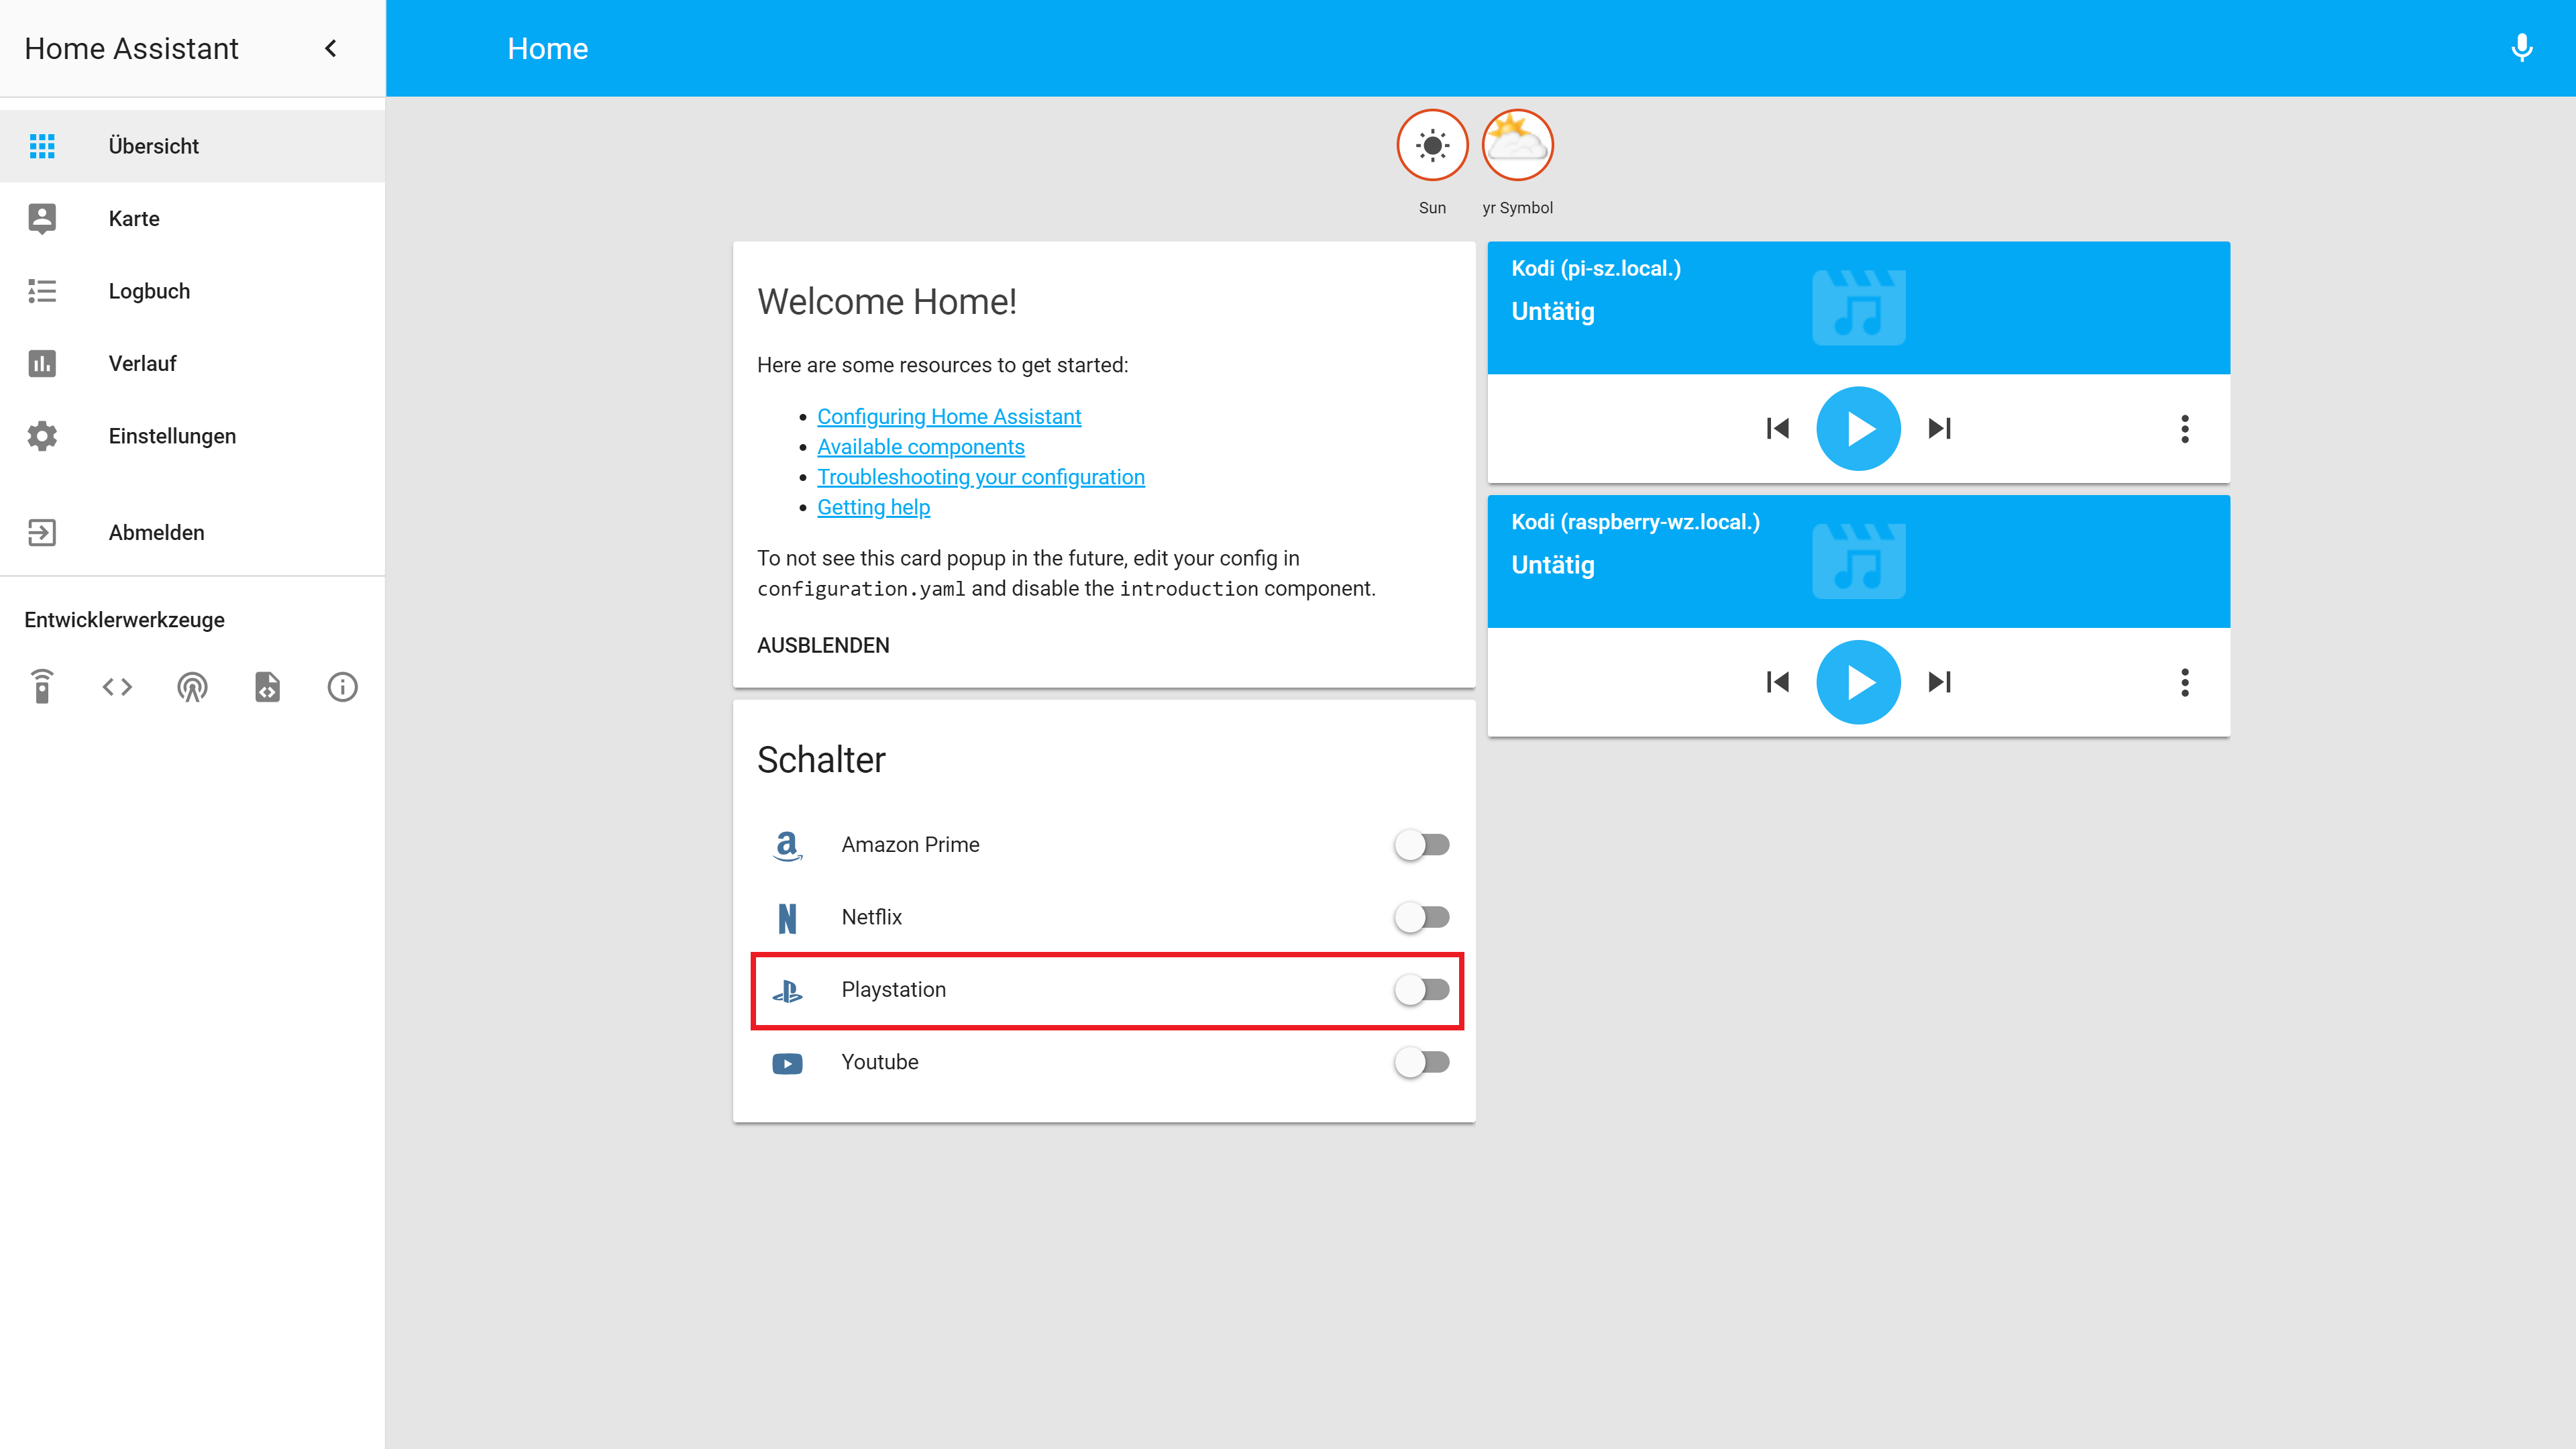
\includegraphics[width=\textwidth]{hass_ui}
    \caption{Weboberfläche des Home Assistant}\label{fig:hass-ui}
\end{figure}

Die Befehle, welche durch Betätigen des Schalters ausgeführt werden,
sind in \ref{sec:aufbau-hassbian} \textit{\nameref{sec:aufbau-hassbian}} unter \autoref{lst:ps4_switch} beschrieben.

Sowohl beim Ein- als auch beim Ausschalten werden zusätzlich zu dem bereits bekannten \texttt{SRCH}-Paket
zwei weitere Arten von UDP-Paketen gesendet.
Das eine enthält den Befehl \texttt{WAKEUP} (\autoref{lst:ps4-wakeup}),
das andere den Befehl \texttt{LAUNCH} (\autoref{lst:ps4-launch}).
Das Feld \texttt{user-credential} (in den Listings gekürzt) ist hierbei immer gleich
und wurde beim initialen Verbindungsaufbau ermittelt.
Laut dem Entwickler werden zwei \texttt{WAKEUP}- und ein \texttt{LAUNCH}-Paket gesendet,
um zu prüfen,
ob die \ac{ps4} bereit ist eine Verbindung anzunehmen.

\lstinputlisting[
    caption=Daten eines WAKEUP-Paketes,
    label=lst:ps4-wakeup
]{ps4_wakeup.udp}

\lstinputlisting[
    caption=Daten eines LAUNCH-Paketes,
    label=lst:ps4-launch
]{ps4_launch.udp}

Der eigentliche Befehl wird dann in der auf die UDP-Pakete folgenden TCP-Verbindung ausgeführt.
Zwar ist diese Verbindung nicht mit TLS verschlüsselt,
die Daten können dennoch nicht ausgelesen werden.
Grund hierfür ist im Quellcode des \textit{ps4-waker} ersichtlich \cite{ps4waker31:online}\cite{ps4waker93:online}.
Die Daten werden dort vor dem Senden auf Anwendungsebene verschlüsselt.
Ein weiterer Blick in den Quellcode zeigt,
dass der Pakettyp (auf Anwendungsebene) durch eine Ganzzahl angegeben wird.
Zusätzlich werden je nach Anwendungsfall ASCII Zeichen oder Ganzzahlen übertragen,
um die gewünschten Befehle auszuführen.
Das Paket eines Standby-Befehls wird beispielsweise wie in \autoref{lst:ps4-standby} erstellt und gesendet (aus \cite{ps4waker31:online}).

\lstinputlisting[
    caption=Erstellen und Senden eines Standby-Befehls,
    label=lst:ps4-standby,
    firstnumber=273
]{ps4_standby.js}

Durch diese Funktionsaufrufe wird ein TCP-Paket der Länge 8 Bytes erstellt,
mit der Zahl 26 gefüllt,
verschlüsselt und gesendet.


\subsection{Ein- und Ausschalten über \textit{Harmony Hub}}\label{sec:durchfuehrung-harmony}
Im Harmony Hub ist zur Nutzung der Playstation 4 eine Aktion namens \enquote{Spielen} konfiguriert.
Zusätzlich zur Spielekonsole wird auch der Fernseher ein- bzw. ausgeschaltet sowie der entsprechende Eingangskanal gewählt.

Zum Einschalten wird der durch den Home Assistant bereitgestelle Schalter genutzt.
Über die emulierte \textit{Hue Bridge} erscheint dieser als Leuchte im Harmony Hub.

Ist die \ac{ps4} eingeschaltet, so kann der Hub eine Bluetooth-Verbindung aufbauen.
Daher ist es zum Ausschalten nicht nötig den Home Assistant zu nutzen.
Der Hub schaltet die Konsole direkt über die Bluetooth-Verbindung aus,
sobald die Aktion beendet wird.

\subsubsection{Einschalten}
In dem Paketmittschnitt sind mehrere TCP-Verbindungen zu erkennen.
An der Kommunikation sind wie erwartet der Harmony Hub, \textit{Hassbian} und die \ac{ps4} beteiligt.
Zusätzlich frägt der Harmony Hub per DNS die IP-Adresse von \nolinkurl{home.myharmony.com} an.
Als Antwort wird auf den Server an mit der URL \nolinkurl{home-myharmony.us-east-1.elasticbeanstalk.com} verwiesen.
Interessant ist hierbei,
dass es sich hierbei um einen von Amazon gehosteten Server für Webanwendungen handelt \cite{AWSElast48:online}.

\textit{Hassbian} und die \ac{ps4} kommunizieren, wie bereits im vorigen Abschnitt untersucht, mittels TCP und UDP.
Der Harmony Hub kommuniziert mit \textit{Hassbian} über HTTP.

Der Ablauf der Kommunikation wird in \autoref{fig:ps-ein-harmony} vereinfacht dargestellt.
Bei HTTP-Verbindungen wird lediglich das HTTP-Paket gezeigt,
der TCP-Rahmen mit Verbindungsaufbau und -abbau wird nicht abgebildet.
Außerdem fehlen in der Abbildung die UDP-Pakete,
welche von \textit{Hassbian} genutzt werden,
um den Status der \ac{ps4} zu Erfragen.
\begin{figure}
    \centering
    \resizebox{\textwidth}{!}{
        \input{assets/uml/ps-ein-harmony.latex}
    }
    \caption{Kommunikation beim Einschalten}
    \label{fig:ps-ein-harmony}
\end{figure}

\newpage



\paragraph{Harmony Hub und Webserver}
Die Verbindungen zum Server dienen vermutlich dazu Informationen über die gestartete Aktion mitzuteilen.
Bei genauerer Betrachtung eines Paketes, welches vom Harmony Hub an den Webserver gesendet wird,
sind verschiedene Besonderheiten zu erkennen.

\begin{figure}[h!]
    \centering
    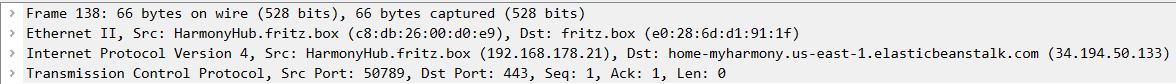
\includegraphics[width=\textwidth]{internet-paket}
    \caption{Paket von Harmony Hub an Webserver}\label{fig:internet-paket}
\end{figure}


\autoref{fig:internet-paket} zeigt die verschiedenen Protokoll-Header, welche ineinander geschachtelt sind.
Die oberste Zeile (\textit{Frame}) steht für das gesamte Paket.
In der zweiten Zeile steht die äußerste Paket-Schicht \textit{Ethernet II}.
Deren Quelladresse ist wie zu erwarten die MAC-Adersse des Harmony Hub.
Als Zieladresse ist jedoch nicht die MAC-Adresse der Webservers,
sondern die der FritzBox angegeben. Dies liegt daran, dass Ethernet lediglich zur Kommunikation im loklen Netzt verwendet wird.
Das Paket wird per Ehternet an die FritzBox gesendet.
Dort wird die \enquote{Ethernet-Nutzlast} (das IP-Paket inklusive TCP) entpackt und über \textit{IPv4} an das eigentliche Ziel weitergeleitet.
Dieses ist als Zieladresse in IP-Header angegeben.

Da die Verbindung an sich verschlüsselt ist, lassen sich aus den übertragenen Daten keine Informationen gewinnen.
Der Zielport des TCP-Headers liefert jedoch einen Hinweis auf die Methode der Übertragung.
Der Port \textit{443} wird standardmäßig für \textit{HTTPS}-Verbindungen genutzt.
Daraus und aus der Tatsache, dass die Verbindung mittels TLS verschlüsselt ist,
lässt sich mit hoher Wahrscheinlichkeit schließen, dass tatsächlich \textit{HTTPS} genutzt wird.


\paragraph{Hassbian und Playstation 4}
Die Kommunikation zwischen \textit{Hassbian} und \ac{ps4} wurde bereits im vorigen Abschnitt betrachtet.
Der Paketmittschnitt zeigt, dass dies, wie zu erwarten, nach dem gleichen Schema abläuft.

\paragraph{Hassbian und Harmony Hub}
Wie erwartet werden auch beim Einschalten HTTP-GET-Requests (siehe \ref{sec:durchfuehrung-aus} \textit{\nameref{sec:durchfuehrung-aus}}) genutzt,
um vom Harmony Hub aus den Status der \ac{ps4} zu erfragen.

Zusätzlich wird ein PUT-Request gesendet, wodurch der Befehl das Gerät einzuschhalten übermittelt wird.
Dieser Request wird an die Adresse \nolinkurl{http://192.168.178.45:8300/api/12345678901234567890/lights/1/state} gesendet.
Der Server ist hier der \textit{Hassbian}, welcher an Port 8300 Befehle an die \textit{Hue Bridge} entgengennimmt.
\texttt{/api/12345678901234567890/lights/1} wählt das zu kontrollierende Gerät aus.
Wie in Kapitel \ref{sec:aufbau-hassbian} \textit{\nameref{sec:aufbau-hassbian}} beschrieben, werden die Geräte nach außen hin als Lichter präsentiert.
Als Nutzdaten enthält das Paket die \autoref{lst:ps4_on-request} gezeigten Daten im JSON-Format.
\lstinputlisting[
    caption=Nutzdaten PUT-Request,
    label=lst:ps4_on-request,
    language=json
]{ps4_on-request.json}
Für diesen Anwendungsfall ist einzig der Wert \lstinline[language=json]{"on": true} von Relevanz.
Mit dem Wert \lstinline[language=json]{"x,y"} könnte bei echten Lampen die Farbe
und mit dem Wert \lstinline[language=json]{"bri"} die Helligkeit gesteuert werden \cite{Coreconc26:online}.

Die Antwort auf den PUT-Request enthält ebenfalls Daten im JSON-Format,
um den Erfolg des Befehls mitzuteilen (siehe \autoref{lst:ps4_on-response}).
\lstinputlisting[
    caption=Nutzdaten PUT-Request,
    label=lst:ps4_on-response,
    language=json
]{ps4_on-response.json}


\subsubsection{Ausschalten}

Da zum Ausschalten der \ac{ps4} der \textit{Hassbian} nicht direkt genutzt wird,
fällt die Netzwerkkommunikation hier deutlich sparsamer aus.

Wieder kommuniziert der Harmony Hub verschlüsselt mit \nolinkurl{home.myharmony.com}.
Außerdem wird der Status der Konsole vom Harmony Hub bei \textit{Hassbian} über die bereits bekannten GET-Requests
und von \textit{Hassbian} bei der Konsole über die SRCH-UDP-Pakete erfragt.

In \autoref{fig:ps-aus-harmony} ist der Ablauf dargestellt.
Im Gegensatz zum vorigen Ablaufdiagramm sind hier die SRCH-UDP-Pakete abgebildet.
Außerdem ist zu den Antworten auf die Statusanfrage notiert,
ob die \ac{ps4} zu diesem Zeitpunkt ein- oder ausgeschaltet ist.


\begin{figure}[ht!]
    \centering
    \resizebox{\textwidth}{!}{
        \input{assets/uml/ps-aus-harmony.latex}
    }
    \caption{Kommunikation beim Ausschalten}
    \label{fig:ps-aus-harmony}
\end{figure}

Aus dem Ablauf ist zu erkennen,
dass die Konsole zwischen dem zweiten GET- und dem zweiten SRCH-Paket ausgeschaltet wurde.
Da dies über einen anderen Kanal (Bluetooth) geschieht,
finden sich im Paketmittschnitt zum Ausschalten selbst keine Nachrichten.